 \section{Creare applicazioni C++}

Non tutti vogliono un'applicazione GIS completa. Talvolta si vuole solamente avereun widget nella propria applicazione che mostri una mappa mentre lo scopo principale dell'applicazione è un altro. Forse un database frontend con un mappa? Questa Sezione fornisce due semplici esempi di scritti da Tim Sutton.
Sono disponibili nell'archivio qgis subversion insieme con altre interessanti guide. L'intero archivio può essere esplorato: 
\filename{https://svn.osgeo.org/qgis/trunk/code\_examples/}

\subsection{Creare un semplice widget mappa}\label{subsec:simple_widget}

Con questa guida si esplora come creare un semplice widget di mappazione. Esso on farà molto - solo caricare uno shape file e mostrarlo in colori casuali. Ma dovrebbe dare un'idea del potenziale per usare QGIS come un componente di mappazione incorporato. Prima di procedere, molti ringraziamenti a Francis Bolduc che ha scritto l'inizio di questo demo. Egli ha gentilmente acconsentito a rendere il suo lavoro pubblicamente disponibile.

Si comincia con la tipica aggiunta del necessario "includes" per la nostra applicazione:

\begin{verbatim}
//
// QGIS Includes
//
#include <qgsapplication.h>
#include <qgsproviderregistry.h>
#include <qgssinglesymbolrenderer.h>
#include <qgsmaplayerregistry.h>
#include <qgsvectorlayer.h>
#include <qgsmapcanvas.h>
//
// Qt Includes
//
#include <QString>
#include <QApplication>
#include <QWidget>
\end{verbatim}

Si usa QgsApplication invece di Qt's QApplication, e si ottengono alcuni benmifici aggiuntivi di vari metodi statici che possono essere usati per localizzare i percorsi della libreria e così via.

Il registro del provider è un singleton che tiene traccia dei plugin del provider di dati vettoriali. Fa tutto il lavoro di caricare i plugin e così via. Il generatore di singolo simbolo è la più basilare classe di simbologia. Genera punti linee o poligoni in un singolo colore che viene scelto predefinitamente in modo casuale (anche se lo si può impostare in modo personalizzato). Ogni layer vettoriale deve avere una simbologia da esso associata.

Il registro del layer di mapp tiene traccia di tutti i layer in uso. La classe del layer vettoriale eredita da maplayer e lo estende ad includere funzionalità specialistiche per dati vettoriali.

Infine il mapcanvas è realmente il nocciolo della questione. E' un widget disegnabile su cui sarà disegnata la mappa.

Ora si può andare oltre alla inizializzazione della nostra applicazione....

\begin{verbatim}
int main(int argc, char ** argv)
{
  // Start the Application
  QgsApplication app(argc, argv, true);

  QString myPluginsDir        = "/home/timlinux/apps/lib/qgis";
  QString myLayerPath         = "/home/timlinux/gisdata/brazil/BR_Cidades/";
  QString myLayerBaseName     = "Brasil_Cap";
  QString myProviderName      = "ogr";

\end{verbatim}

Così ora abbiamo un'applilcazione qgs e abbiamo definito alcue varibili. Dato che ho testato su Ubuntu 8.10, specifico qui le posizione dei plugin del provider vettoriale come nella mia directory di istallazione sviluppo. Probabilmente avrebbe più senso in generale tenere le lilbrerie QGIS libs in uno dei percorsi di ricerca delle library standard del vostro sistemas (ad es. /usr/lib) ma per ora andrà bene anche così.

Le prossime due variabili definite qui indicano solo il file shape che si userà (e qui dovreste sostituire i vostri dati).

Il nome del provider è importante - dice a QGIS che provider di dati usare per caricare il file. Tipicamente si userà 'ogr' o 'postgres'.

Ora possiamo creare il ayer oggetto.

\begin{verbatim}
  // Instantiate Provider Registry
  QgsProviderRegistry::instance(myPluginsDir);
\end{verbatim}

Prima si inizializza il registro del provider. E' una classe singleton quindi si usa un'istanza di chiamata statica e si passa il percorso di ricerca della library del provider. Appena inizializzato scansionerà questo percorso alla ricerca di lbrerie del provider.

Ora si crea un layer...

\begin{verbatim}
  QgsVectorLayer * mypLayer =
      new QgsVectorLayer(myLayerPath, myLayerBaseName, myProviderName);
  QgsSingleSymbolRenderer *mypRenderer = new
QgsSingleSymbolRenderer(mypLayer->geometryType());
  QList <QgsMapCanvasLayer> myLayerSet;

  mypLayer->setRenderer(mypRenderer);
  if (mypLayer->isValid())
  {
    qDebug("Layer is valid");
  }
  else
  {
    qDebug("Layer is NOT valid");
  }

  // Add the Vector Layer to the Layer Registry
  QgsMapLayerRegistry::instance()->addMapLayer(mypLayer, TRUE);
  // Add the Layer to the Layer Set
  myLayerSet.append(QgsMapCanvasLayer(mypLayer, TRUE));

\end{verbatim}

Il codice è adeguatamente auto esplicativo qui. Si crea un layer usando le variabili definite prima. Poi si assegna al layer un generatore di immagini. Quando si crea un generatore di immagini, dobbiamo specificare il tipo di geometria, cosa che si fa chiedendo allo stato vettoriale il suo tipo di geometria. Poi si aggiunge il layer ad un set di layer (che è usato da QgsMapCanvas per tenere traccia di quali layer generare graficamente e in che ordineo) e al registro di maplayer. Infine ci si assicura che il layer sarà visibile.
Ora si crea un map canvas sul quale disegnare il layer.

\begin{verbatim}
  // Create the Map Canvas
  QgsMapCanvas * mypMapCanvas = new QgsMapCanvas(0, 0);
  mypMapCanvas->setExtent(mypLayer->extent());
  mypMapCanvas->enableAntiAliasing(true);
  mypMapCanvas->setCanvasColor(QColor(255, 255, 255));
  mypMapCanvas->freeze(false);
  // Set the Map Canvas Layer Set
  mypMapCanvas->setLayerSet(myLayerSet);
  mypMapCanvas->setVisible(true);
  mypMapCanvas->refresh();

\end{verbatim}

Once again there is nothing particularly tricky here. We create the canvas
and then we set its extents to those of our layer. Next we tweak the canvas a bit
to draw antialiased vectors. Next we set the background colour, unfreeze the
canvas, make it visible and then refresh it.

\begin{verbatim}
  // Start the Application Event Loop
  return app.exec();
}

\end{verbatim}

In the last step we simply start the Qt event loop and we are all done. You
can check out, compile and run this example using cmake like this:

\begin{verbatim}
svn co
https://svn.osgeo.org/qgis/trunk/code_examples/1_hello_world_qgis_style
cd 1_hello_world_qgis_style
mkdir build
#optionally specify where your QGIS is installed (should work on all
platforms)
#if your QGIS is installed to /usr or /usr/local you can leave this next step
out
export LIB_DIR=/home/timlinux/apps
cmake ..
make
./timtut1
\end{verbatim}

When we compile and run it here is what the running app looks like:

\begin{figure}[ht]
   \begin{center}
   \caption{Simple C++ Application \osxcaption}\label{fig:cpp1_application}\smallskip
   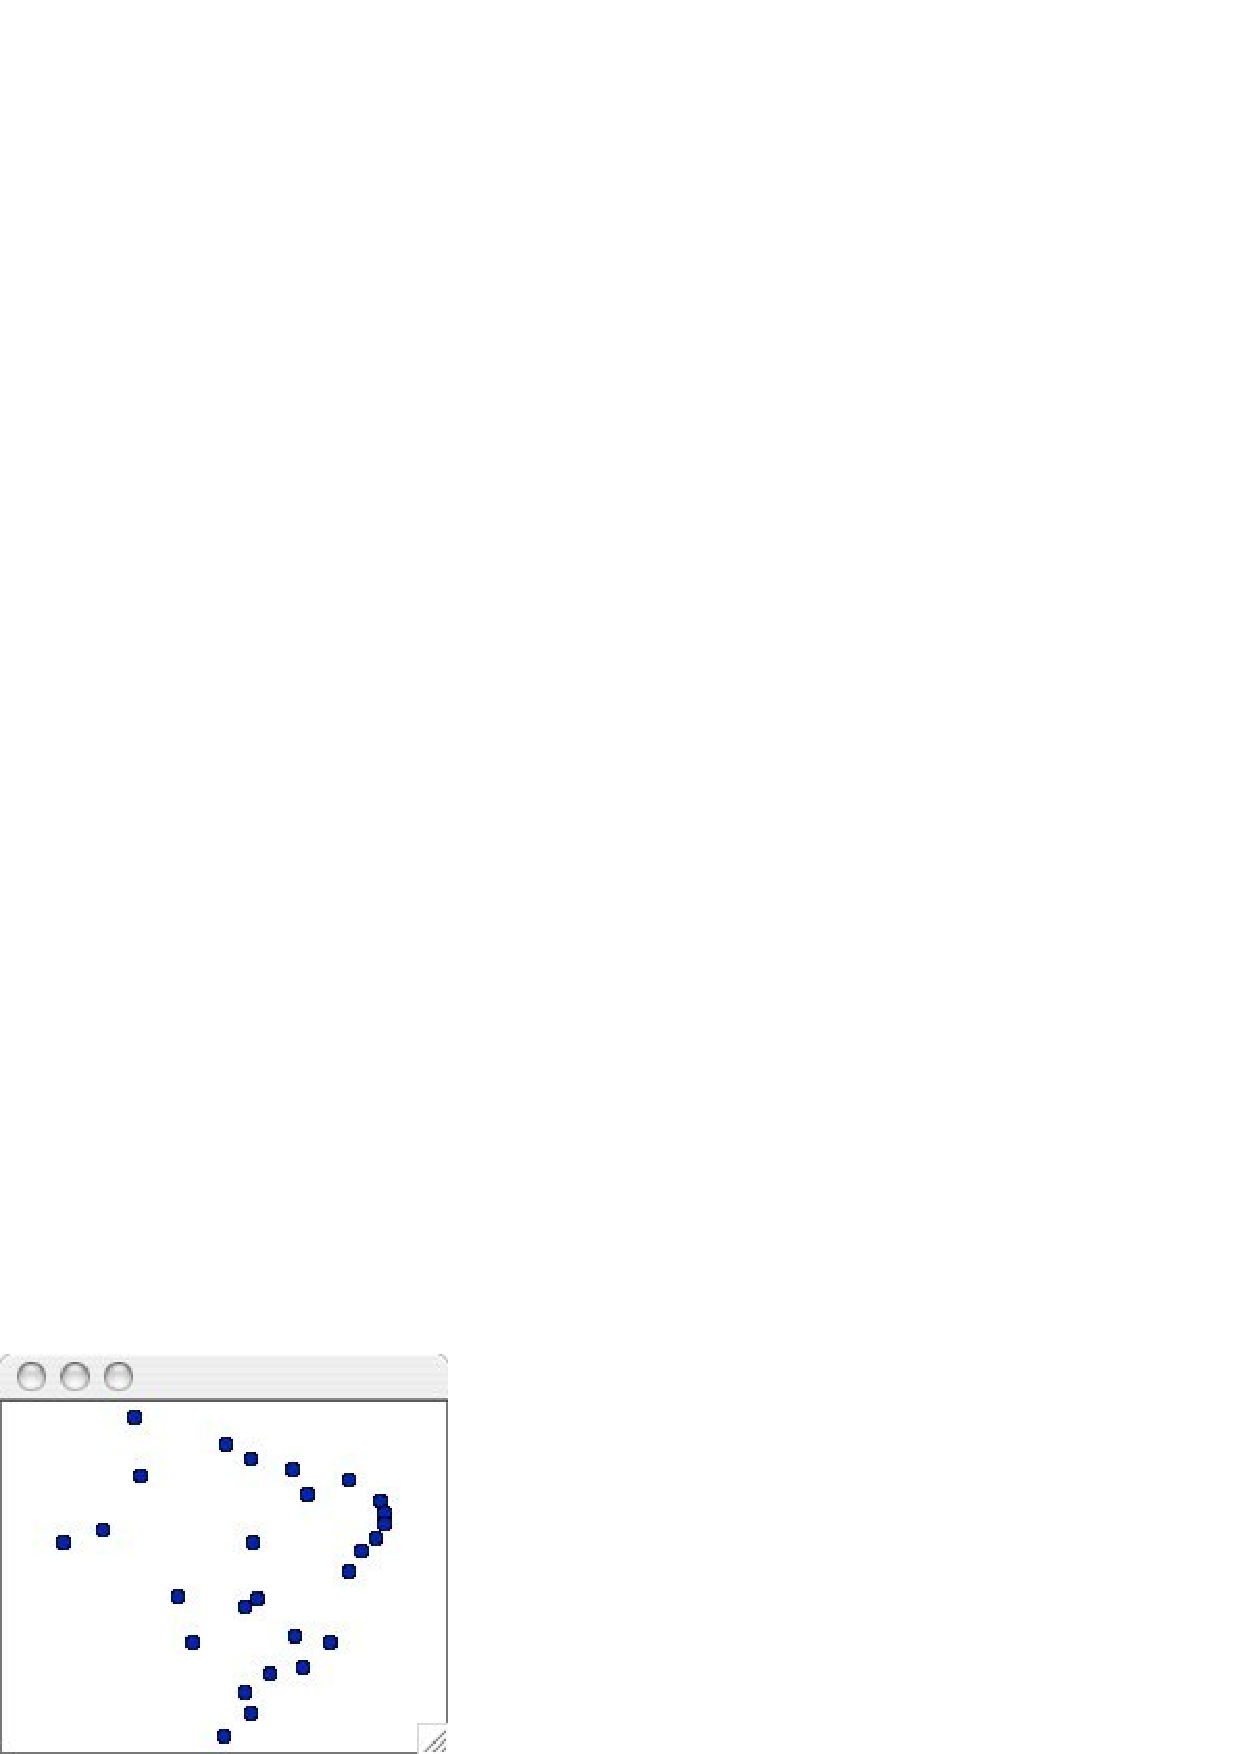
\includegraphics[clip=true]{cpp1_application}
\end{center}
\end{figure}

\subsection{Working with QgsMapCanvas}

In Section~\ref{subsec:simple_widget} we showed you the usage of the
QgsMapCanvas api to create a simple application that loads a shapefile and
displays the points in it. But what good is a map that you can't interact
with? 

In this second tutorial I will extend the last tutorial by making it a
QMainWindow application with a menu, toolbar and canvas area. We show you how
to use QgsMapTool - the base class for all tools that need to interact with
the map canvas.
The purpose is to provide a demonstrator project, so I wont promise to write the most
elegant or robust C++ code. The project will provide 4 toolbar icons for

\begin{itemize}
 \item loading a map layer (layer name is hard coded in the application
 \item zooming in
 \item zooming out
 \item panning
\end{itemize}

In the working directory for the tutorial code you will find a number of files
including c++ sources, icons and a simple data file under data. There is also
the .ui file for the main window.

\textbf{Note:} You will need to edit the .pro file in the above svn directory to
match your system.

Since much of the code is the same as the previous tutorial, I will focus on
the MapTool specifics - the rest of the implementation details can be
investigated by checking out the project form SVN. A QgsMapTool is a class that
interacts with the MapCanvas using the mouse pointer. QGIS has a number of
QgsMapTools implemented, and you can subclass QgsMapTool to create your own. In
mainwindow.cpp you will see I include the headers for the QgsMapTools near the
start of the file:

\begin{verbatim}
     //
     // QGIS Map tools
     //
     #include "qgsmaptoolpan.h"
     #include "qgsmaptoolzoom.h"
     //
     // These are the other headers for available map tools 
     // (not used in this example)
     //
     //#include "qgsmaptoolcapture.h"
     //#include "qgsmaptoolidentify.h"
     //#include "qgsmaptoolselect.h"
     //#include "qgsmaptoolvertexedit.h"
     //#include "qgsmeasure.h"
\end{verbatim}

As you can see, I am only using two types of MapTool subclasses for this
tutorial, but there are more available in the QGIS library. Hooking up our
MapTools to the canvas is very easy using the normal Qt4 signal/slot mechanism:

\begin{verbatim}
     //create the action behaviours
     connect(mActionPan, SIGNAL(triggered()), this, SLOT(panMode()));
     connect(mActionZoomIn, SIGNAL(triggered()), this, SLOT(zoomInMode()));
     connect(mActionZoomOut, SIGNAL(triggered()), this, SLOT(zoomOutMode()));
     connect(mActionAddLayer, SIGNAL(triggered()), this, SLOT(addLayer()));
\end{verbatim}

Next we make a small toolbar to hold our toolbuttons. Note that the mpAction*
actions were created in designer.

\begin{verbatim}
     //create a little toolbar
     mpMapToolBar = addToolBar(tr("File"));
     mpMapToolBar->addAction(mpActionAddLayer);
     mpMapToolBar->addAction(mpActionZoomIn);
     mpMapToolBar->addAction(mpActionZoomOut);
     mpMapToolBar->addAction(mpActionPan);
\end{verbatim}

Thats really pretty straightforward Qt stuff too. Now we create our three map
tools:

\begin{verbatim}
     //create the maptools
     mpPanTool = new QgsMapToolPan(mpMapCanvas);
     mpPanTool->setAction(mpActionPan);
     mpZoomInTool = new QgsMapToolZoom(mpMapCanvas, FALSE); // false = in
     mpZoomInTool->setAction(mpActionZoomIn);
     mpZoomOutTool = new QgsMapToolZoom(mpMapCanvas, TRUE ); //true = out
     mpZoomOutTool->setAction(mpActionZoomOut);
\end{verbatim}

Again nothing here is very complicated - we are creating tool instances, each
of which is associated with the same mapcanvas, and a different QAction. When
the user selects one of the toolbar icons, the active MapTool for the canvas is
set. For example when the pan icon is clicked, we do this:

\begin{verbatim}
    void MainWindow::panMode()
    {
       mpMapCanvas->setMapTool(mpPanTool); 
    }
\end{verbatim}

\begin{figure}[ht]
   \begin{center}
   \caption{QMainWindow application with a menu, toolbar and canvas area
\osxcaption}\label{fig:cpp2_application}\smallskip
   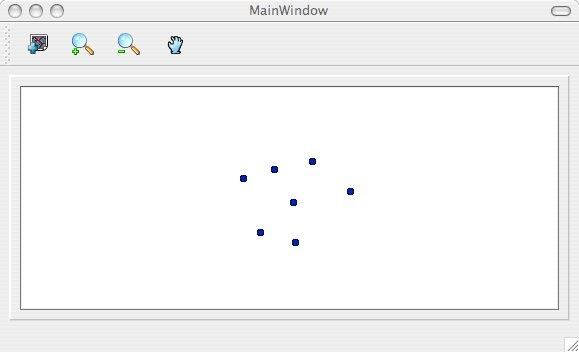
\includegraphics[clip=true, width=\textwidth]{cpp2_application}
\end{center}
\end{figure}

\minisec{Conclusion}

As you can see extending our previous example into something more functional
using MapTools is really easy and only requires a few lines of code for each
MapTool you want to provide.

You can check out and build this tutorial using SVN and CMake using the following steps:

\begin{verbatim}
svn co https://svn.osgeo.org/qgis/trunk/code_examples/2_basic_main_window
cd 2_basic_main_window
mkdir build
#optionally specify where your QGIS is installed (should work on all platforms)
#if your QGIS is installed to /usr or /usr/local you can leave this next step out
export LIB_DIR=/home/timlinux/apps
cmake ..
make
./timtut2
\end{verbatim}


